\section{Introduction}
Handwritten digit recognition is the ability for a computer to receive and interpret handwritten input. There is a great interest in this area due to many potential application capable of using this. Examples could be analyzing large number documents such as at post offices for sorting purposes, or for processing handwritten forms in which the use of a computer rather doing it manually would be highly beneficial.  \\

The purpose of this report is the create a digit recognizer based on two different methods.  The methods tested in this report are kNN and SVM, as they prior to this have shown reasonable results.\\

The data used for training and testing purposes is gained from the students participated in the class.  Each student were to fill out 10 sheets of paper, each with different digits from 0 to 9 an example is depicted in figure \ref{fig:handwriten_digits}. 

\begin{figure}[H]
\centering
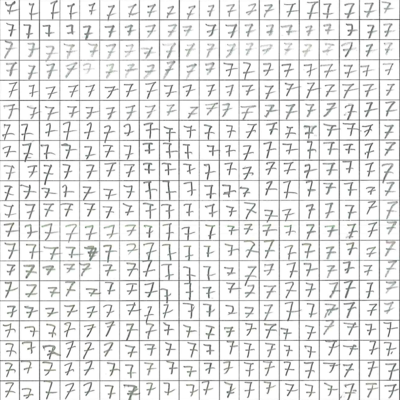
\includegraphics[width = 0.5\textwidth]{img/cropY2016G2M1-100-7.png}
\caption{Handwritten digits}
\label{fig:handwriten_digits}
\end{figure}

Each of these sheets of papers are then scanned with DPI resolutions such as 100,200,300 and then processed on for training and testing purposes. 
\newpage